\chapter{Graphic User Interface}
\label{c:gui}

%-----------------------------------------------------------------
\section{GUI Installation}
\label{s:gui.install}

There are a number of python modules needed for the GUI:
\begin{example}
  tkinter
  ttk (may be called pyttk)
  pexpect         # If using pexpect instead of ctypes.
  matplotlib, cycler, dateutil, tkagg
\end{example}
Note: The GUI uses the TkAgg backend for matplotlib. There may be a problem with Python finding the
TkAgg backend. On the mac, using macports, the solution is to install matplotlib with the
\vn{tkinter} variant. Something like:
\begin{example}
  sudo port uninstall py36-matplotlib           # May not be needed.
  sudo port install  py36-matplotlib +tkinter   # This is when using Python version 3.6
\end{example}
For more information see:
\begin{example}
  https://matplotlib.org/tutorials/introductory/usage.html#backends
\end{example}

If one of the modules is missing, python will generate an error message. For example:
\begin{example}
> python ../../gui/main.py
Exception in Tkinter callback
Traceback (most recent call last):
  File "/opt/local/Library/Frameworks/Python.framework/Versions/3.7/lib/python3.7/tkinter/__init__.py", line 1705, in __call__
    return self.func(*args)
  File "../../gui/main.py", line 372, in param_load
    from tao_interface import tao_interface
  File "/Users/dcs16/Bmad/bmad_dist/tao/gui/tao_interface.py", line 4, in <module>
    from tao_pipe import tao_io
  File "/Users/dcs16/Bmad/bmad_dist/tao/python/tao_pexpect/tao_pipe.py", line 14, in <module>
    import pexpect
ModuleNotFoundError: No module named 'pexpect'
\end{example}
Notice that the last line shows that the pexpect module is needed.

How to install missing modules on the mac: [Note: The exact installation commands will depend upon
which version of python is being used. Use the "python --version" command to see what version you
are using.

Using macports and python 3.6:
\begin{example}
  sudo port install py36-tkinter
  sudo port install py36-pexpect
\end{example}

Using pip (or pip3):
\begin{example}
  sudo pip install pytkk
  sudo pip install pexpect
\end{example}

WARNING: it can be dangerous to use pip to install/modify modules in your system python.
A much safer way to install the modules you need is to set up a python virtual environment.
On Linux, you may also be able to find versions of the required modules in your system package manager,
which are tailored to your Linux distribution and will not break your system python.

%-----------------------------------------------------------------
\subsection{Installation Troubleshooting}
\label{s:gui.trouble}

Got error:
\begin{example}
  ImportError: cannot import name ‘_tkagg'
\end{example}

Solution: Uninstall and then reinstall matplotlib. For example, if using pip:
\begin{example}
  sudo pip uninstall matplotlib
  sudo pip install matplotlib
\end{example}

%-----------------------------------------------------------------
\subsection{Developer Setup}
\label{s:gui.develop}

For GUI development, it may be desireable to specify a local build tree as the place for the python
scripts to find the \tao executable and other modules. To accomplish this, set the environmental
variable ACC_LOCAL_ROOT to the base directory of your local build tree.


%-----------------------------------------------------------------
\section{Starting the GUI}
\label{s:gui.startup}
From your system shell, you can execute the gui with the command
\begin{example}
  python -m pytao.gui
\end{example}
either from the \texttt{tao/python} directory, or from anywhere on your system if the pytao package is installed somewhere in your python path.  You can also specify any of the command line options that tao supports.  For example,
\begin{example}
  python -m pytao.gui -init_file ~/bmad_dist/tao/examples/cesr/tao.init -rf_on
\end{example}
This will prefill the settings for \texttt{init_file} and \texttt{rf_on}.
The GUI starts with the window shown in Figure \ref{fig:startup}.
From here, all of the command-line settings that Tao supports can be set (settings that are left blank are omitted when Tao is started).

Towards the bottom of the window are some settings that are specific to the GUI.  The "Interface to Tao" setting controls whether the ctypes or pexpect backend for communicating with Tao will be used.
Below it, the "Shared Library" or "Tao executable" setting points the GUI to the correct executable or shared object library to use.
In most cases, the GUI will prefill this box by referencing the ACC_LOCAL_ROOT and ACC_ROOT_DIR environmental variables.

Finally, the font size can be set as desired.
Hitting Enter/Return while the font size box is in focus will adjust the font size of the startup window to give the user a sense of what the chosen font size will look like.

Once all of the startup settings have been set, clicking "Start Tao" will initialize Tao and bring the user to the main GUI window.
\begin{figure}
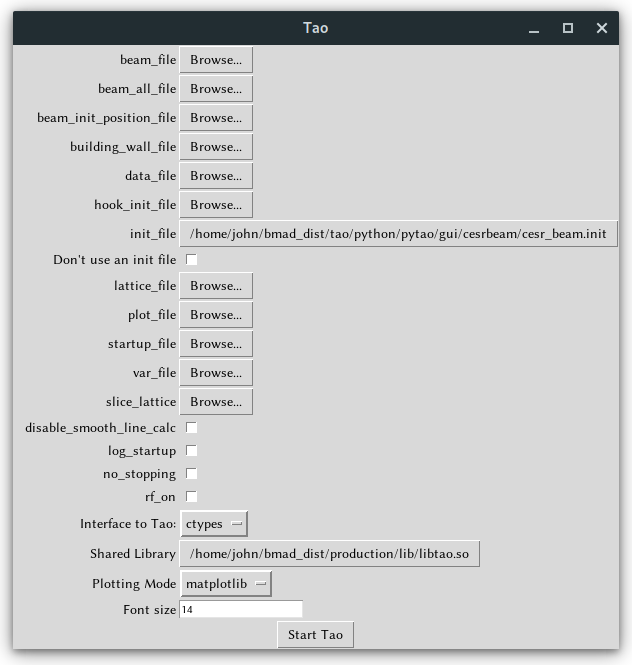
\includegraphics[width=8cm]{figures/startup.png}
\centering
\caption{The GUI startup window.  In this example, the init file that tao should use has been specified.}
\label{fig:startup}
\end{figure}

%--------------------------------------------------------------

\subsection{GUI Initialization File}
\label{s:gui.init.file}

To speed up the initialization process, you can make an init file for the GUI.  This file should be called "gui.init", and it should be in the same directory from which you initialize the GUI.

gui.init should have each option on a separate line, and each option should be listed in the form "parameter:value".  For example, the text below would constitute a good gui.init file:

\begin{example}
  #MY GUI INIT FILE
  beam_file:/path/to/beam/file
  data_file:/path/to/data/file
  #THIS IS A COMMENT
  disable_smooth_line_calc:T
  rf_on:T
  tao_exe:/path/to/executable
\end{example}

The order in which you list options in gui.init is not important.

File paths should be specified in full to be safe, but you can specify paths relative to the directory from which you launch main.py.  For example, "/home/username/file", "subfolder/my_file", and "../../path/to/another/file" would all be acceptable file paths.  You can also use your environmental variables and "\textasciitilde{}", as in "\textasciitilde{}/Documents/my_file" and "\$DIST_BASE_DIR/tao/file".

Logic (true/false) options may be specified by T/F or True/False.

You can also include comments with \#.  Any line with \# as its first non-whitespace character will be considered a comment and ignored.

%-----------------------------------------------------------------

\section{The Main GUI Window}
\label{s:gui.root.window}

The main window for the GUI is shown in Figure \ref{fig:root.window}.
\begin{figure}
\centering
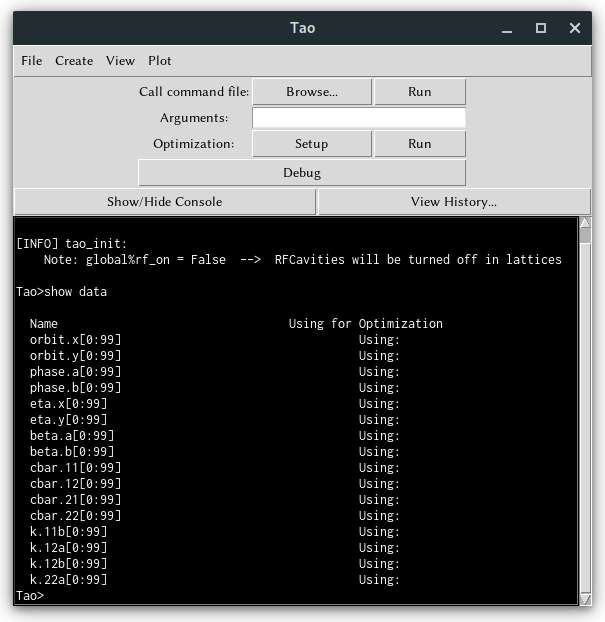
\includegraphics[width=8cm]{figures/root_window.png}
\caption{The main GUI window, showing the results of \texttt{show data} on the console.}
\label{fig:root.window}
\end{figure}
From here, the user has access to all of the GUI's features.
Command files can be called by browsing for them and then clicking "Run", with arguments specified in the "Arguments" below.
In the future, the user will also be able to set up and run optimization routines from this window, although this feature is not currently available.

The main window also has a console, where commands can be run in Tao exactly like in regular Tao.
The console will also display warning messages if a command produces an error.

%-----------------------------------------------------------------

\section{Global Variables}
\label{s:gui.global.variables}

Global variables in Tao can be viewed and modified from the global variables window as shown in Figure \ref{fig:gui.global.variables}.
Once you have editted the global variables, clicking the "Set Global Variables" button will set the variables in Tao as appropriate.

\begin{figure}
\centering
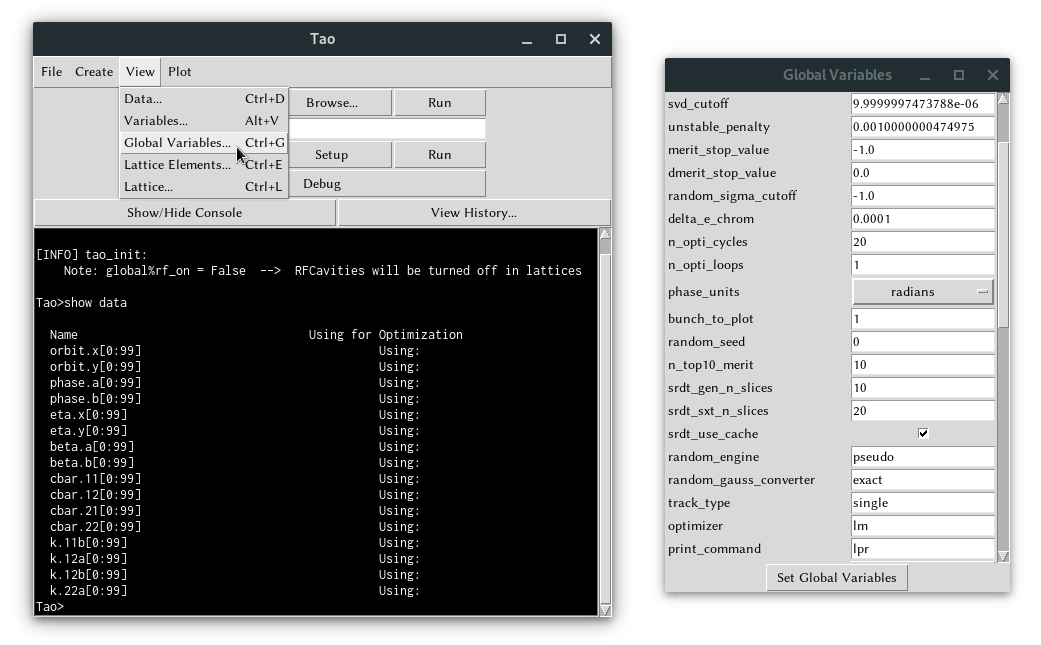
\includegraphics[width=10cm]{figures/globals.png}
\caption{View and edit global variables with the Global Variables window.}
\label{fig:gui.global.variables}
\end{figure}

%-----------------------------------------------------------------
\section{Data}
\label{s:gui.data}

The GUI provides several windows for viewing and editing data arrays.

\subsection{Viewing Data}
\label{s:gui.data.view}

Figure \ref{fig:gui.data.view} shows the various windows that the GUI provides for viewing data and making minor changes to data arrays.
\begin{figure}
\centering
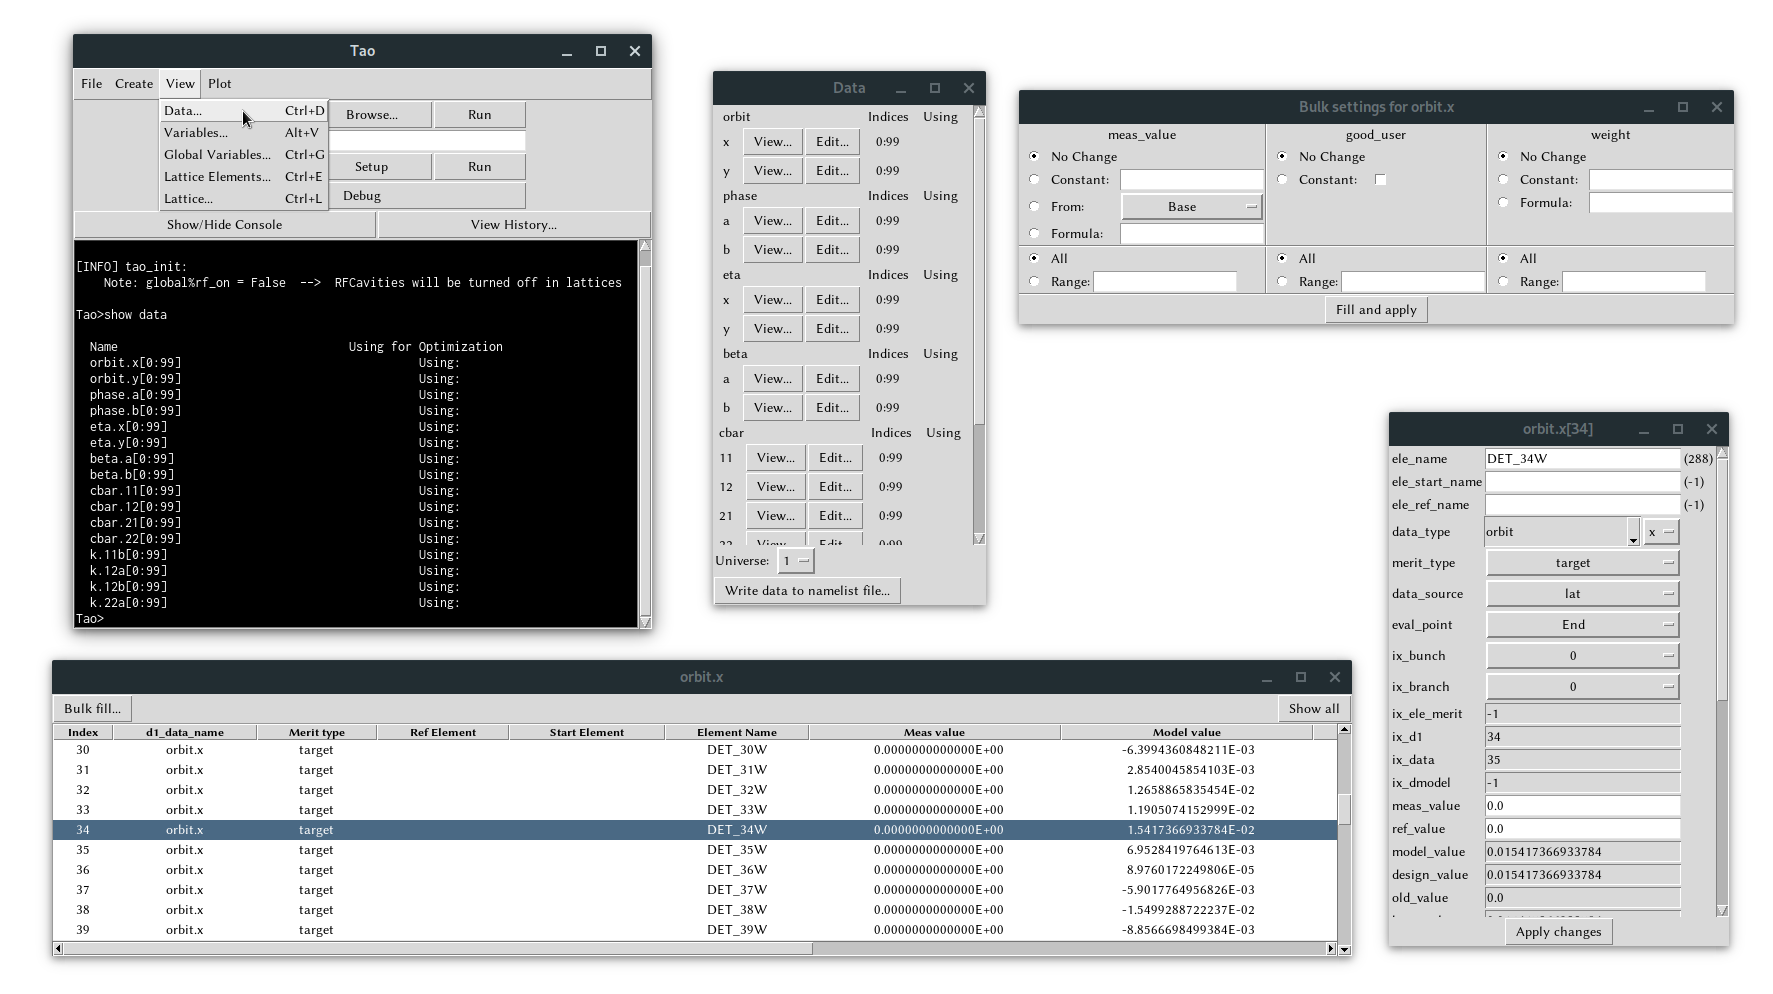
\includegraphics[width=12cm]{figures/view_data.png}
\caption{The GUI's data viewing windows.
Top left: the Tao root window and the menu shortcut for viewing data.
Top middle: The d2_data_array window, which list the currently defined d2_data_arrays for each universe.
This window also includes links to view and edit (see section \ref{s:gui.data.edit}) existing d1_data_arrays.
Bottom left: The d1_data_array window (in this case for orbit.x), showing all of the datums in the array orbit.x.
Bottom right: The individual datum window (in this case for orbit.x[34]) displaying detailed datum properties and allowing the user to edit some of these properties.
Top right: The bulk edit window (in this case for orbit.x) providing controls to quickly edit a few key properties for multiple datums in a d1_data_array.}
\label{fig:gui.data.view}
\end{figure}

The d2_data_array window (top middle in Figure \ref{fig:gui.data.view}) displays all data arrays for a given universe.
To view any existing d1_data_array, click on its "View" button.
This window also provides the ability to edit any existing data array in detail (see Section \ref{s:gui.data.edit}), as well as functionality for writing existing data to a namelist (see Section \ref{s:gui.namelist}).

The d1_data_array window (bottom left in Figure \ref{fig:gui.data.view}) allows the user to view an existing d1_data_array.
This window displays important properties of each datum in the array, such as element name, meas, model, and design values, and weight, in a scrollable table.
To view a datum in detail, double click on its row in the d1_data_array window.
This will open the individual datum window for that datum, displaying all of its properties and allowing some of them to be editted.

The d1_data_array window also allows the user to edit a few key properties of the datums in the array all at once using the bulk settings window (top right in Figure \ref{fig:gui.data.view}).
This window is accessed by clicking on the "Bulk fill" button in the d1_data_array window.
From here, the meas_value, good_user, and weight settings for the datums in the array can be edited in bulk.
Changes may be applied to every datum in the array, or to only a specific range of datums using the range specifier.
Once the desired settings have been specified, clicking the "Fill and apply" button will edit the d1_data_array as necessary, and changes will be reflected in the d1_data_array window.

\subsection{Creating and Editing Data}
\label{s:gui.data.edit}

The GUI also supports the creation of data arrays on the fly through the create data window.
This window can be accessed as shown in figure \ref{fig:gui.create.data.d2}.
\begin{figure}
\centering
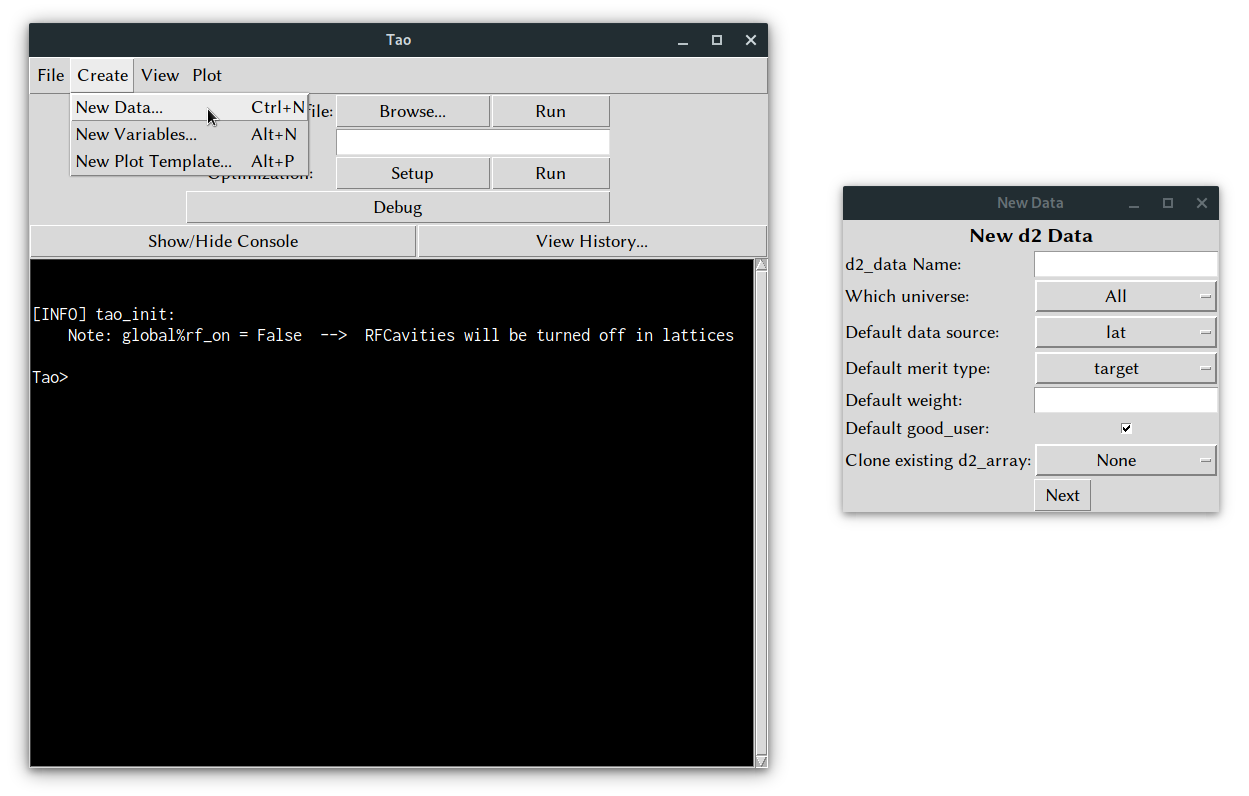
\includegraphics[width=12cm]{figures/create_d2.png}
\caption{Left: the data creation window can be accessed from the root window's menubar. \\
Right: The first pane of the data creation window.}
\label{fig:gui.create.data.d2}
\end{figure}
In the first pane of the data creation window, the user can input the desired settings for the new d2_data_array.
The user can also select and existing d2_data_array to clone.
This will copy the d2 properties of that array, as well as the d1 properties and all of the datums for each d1 array.
Once this information has been input, the user can hit the "Next" button to go to the d1_data_array pane.

The d1_array pane of the data creation window is where most of the data array's properties are set.
This pane is shown in Figure \ref{fig:gui.create.data.d1}.
\begin{figure}
\centering
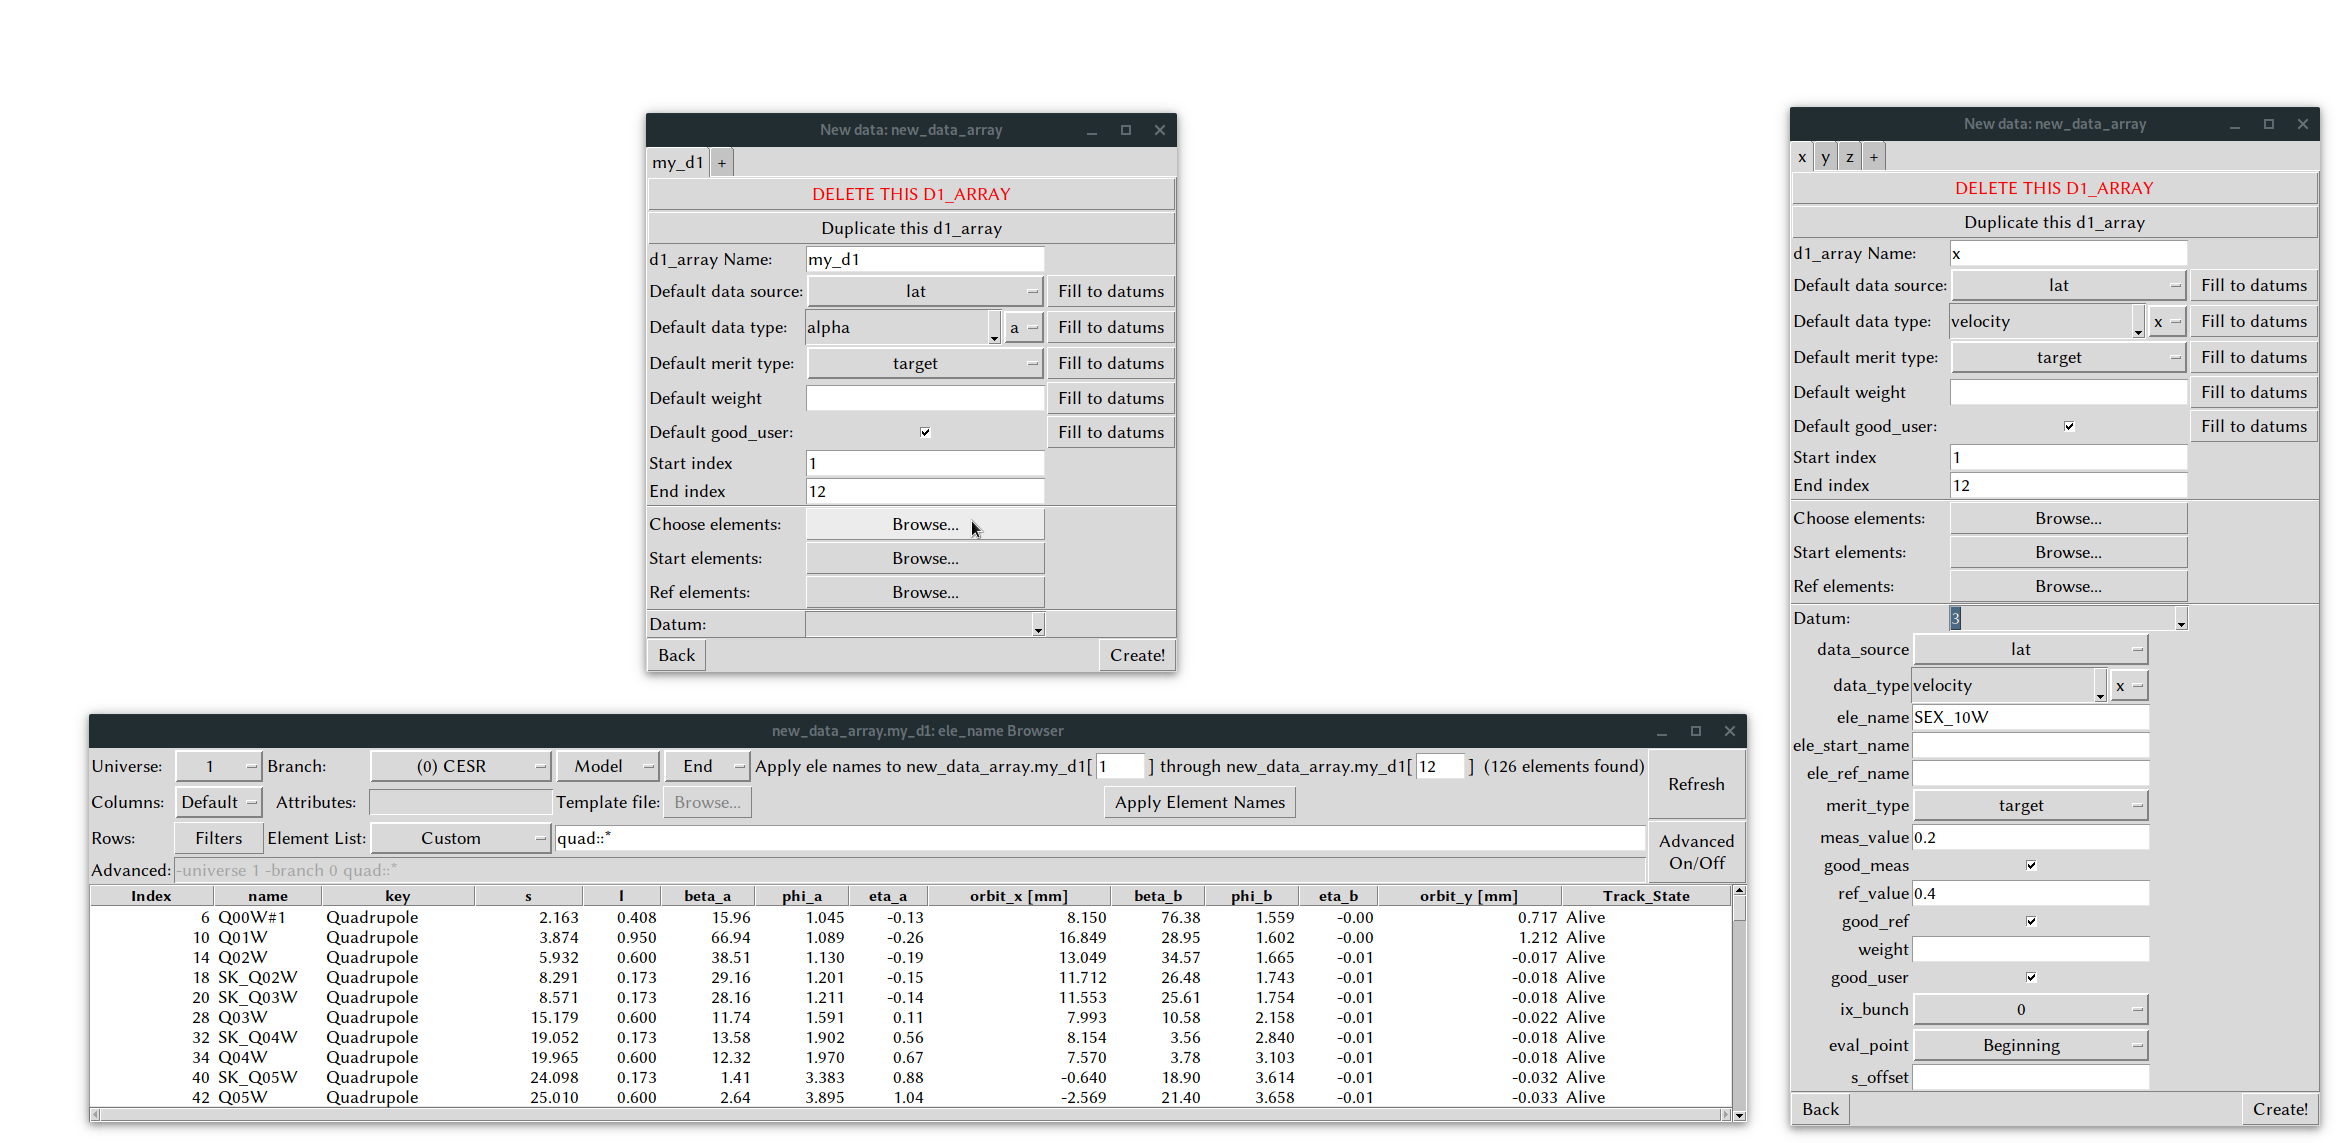
\includegraphics[width=12cm]{figures/create_d1.png}
\caption{The d1_array pane of the data creation window.  Top left: Here, only one d1_array has been created (called my_d1), its default data type has been set to alpha.a, and the start and end indices have been set to 1 and 12 respectively.  \\
Bottom left: the lattice browser for the ele_names that will be used with my_d1.
Right: Here, the user has defined three d1_arrays: x, y, and z.
The data type for new_data_array.x has been set to velocity.x, and the start and end indices have been set to 1 and 12.
Here, the user is currently editing new_data_array.x[3], where the meas value has been set to 0.2 and the ref value has been set to 0.4.}
\label{fig:gui.create.data.d1}
\end{figure}
The d1_array pane of the data creation window displays each d1_array in its own tab.
To add a tab, click on the "+" tab at the top of the window.
Tabs can also be removed by navigating to them and then clicking on their delete button.
An existing tab can also be duplicated by clicking on the duplicate button right under the delete button.
This may be useful if you want to define several d1_arrays with many of the same properties, but want them each to have a different data type, for example.

The next section of the window holds the d1-level settings for the array.
Here, the d1 name, start index, and end index can be set, as well as the default data_source, data_type, merit type, weight, and good user value for the d1_array.

The next section allows the users to set the ele_name, ele_start_name, and ele_ref_name for the d1_array en-masse.
Clicking on these buttons will bring up the lattice browser window (bottom left in Figure \ref{fig:gui.create.data.d1}).
This window is essentially identical to the main lattice window for the GUI (see Section \ref{s:gui.lat}), with a few additions.
Towards the top right of the window, the user can specify which indices to read the element names into.
Clicking "Apply Element Names" will then write the ele names that are currently in the table sequentially into the d1_array's datums.
In the example shown in Figure \ref{fig:gui.create.data.d1}, new_data_array.my_d1[1]|ele_name will be set to "Q00W\#1", new_data_array.my_d1[2]|ele_name will be set to "Q01W", and so on.
If there are more elements in the table than there are datums to write to, the table will be truncated and only the first elements in the table will be used.
If there are less elements in the table than there are datums to write to, the elements in the table will be looped through so that each datum gets an element name.

The bottom portion of the d1_array pane of the data creation window allows the user to set the properties of the individual datums in the array.
Once a start and end index have been specified, the "Datum" drop down menu will be populated with all of the datum indices.
Selecting an index will bring up the datum settings for that datum, as shown in the right of Figure \ref{fig:gui.create.data.d1}.
Note that any settings that have a d1-level default value are automatically filled in.
Once the user edits a property of a datum, that property will no longer be auto-filled from the d1-level default settings, even if those default values are subsequently edited.
If the user wants to explicitly fill a d1 setting to that d1_array's datums, they may do so with the corresponding "Fill to datums" button.

Once all of the data settings have been adjusted as necessary, the user must click the "Create" button to create the d2_array in Tao.  Doing so will close the data creation window.

The data creation window can also be accessed from the d2_data window discussed in Section \ref{s:gui.data.view}.
Clicking on the "Edit" button for any d2 array will load that array into the data creation window, just as if the user had cloned that array from the d2 pane of the data creation window.
This is shown in Figure \ref{fig:gui.edit.data}
\begin{figure}
\centering
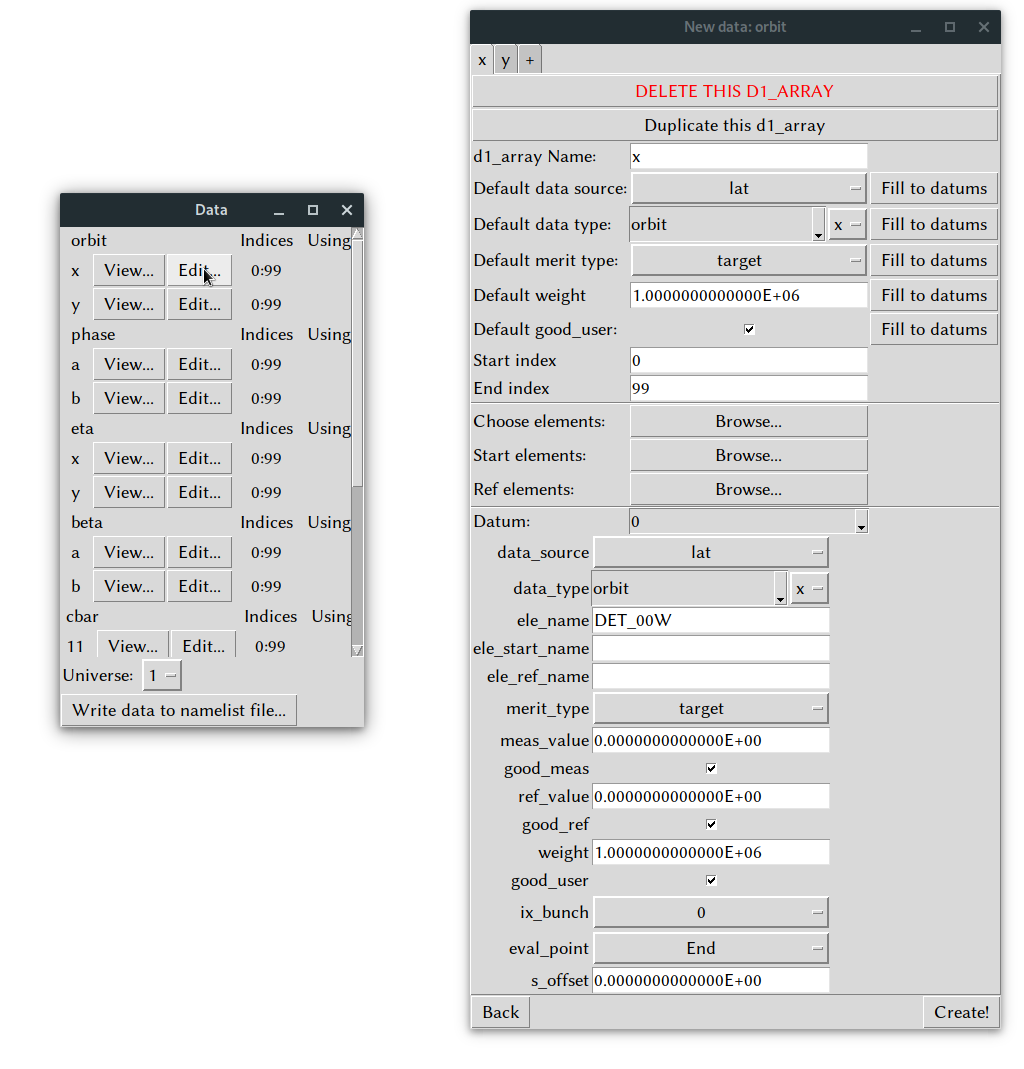
\includegraphics[width=12cm]{figures/edit_data.png}
\caption{Editting an existing d2_data_array.}
\label{fig:gui.edit.data}
\end{figure}
Note that any changes made in the data creation window will not take effect in Tao until the user clicks the "Create" button.
For example, clicking the delete button for the orbit.x array would not actually delete the array in Tao until the user clicks "Create".

%-----------------------------------------------------------------
\section{Variables}
\label{s:gui.variables}

Variables are viewed and edited in the GUI almost exactly the same as data, as shown in Figure \ref{fig:gui.variables}.
\begin{figure}
\centering
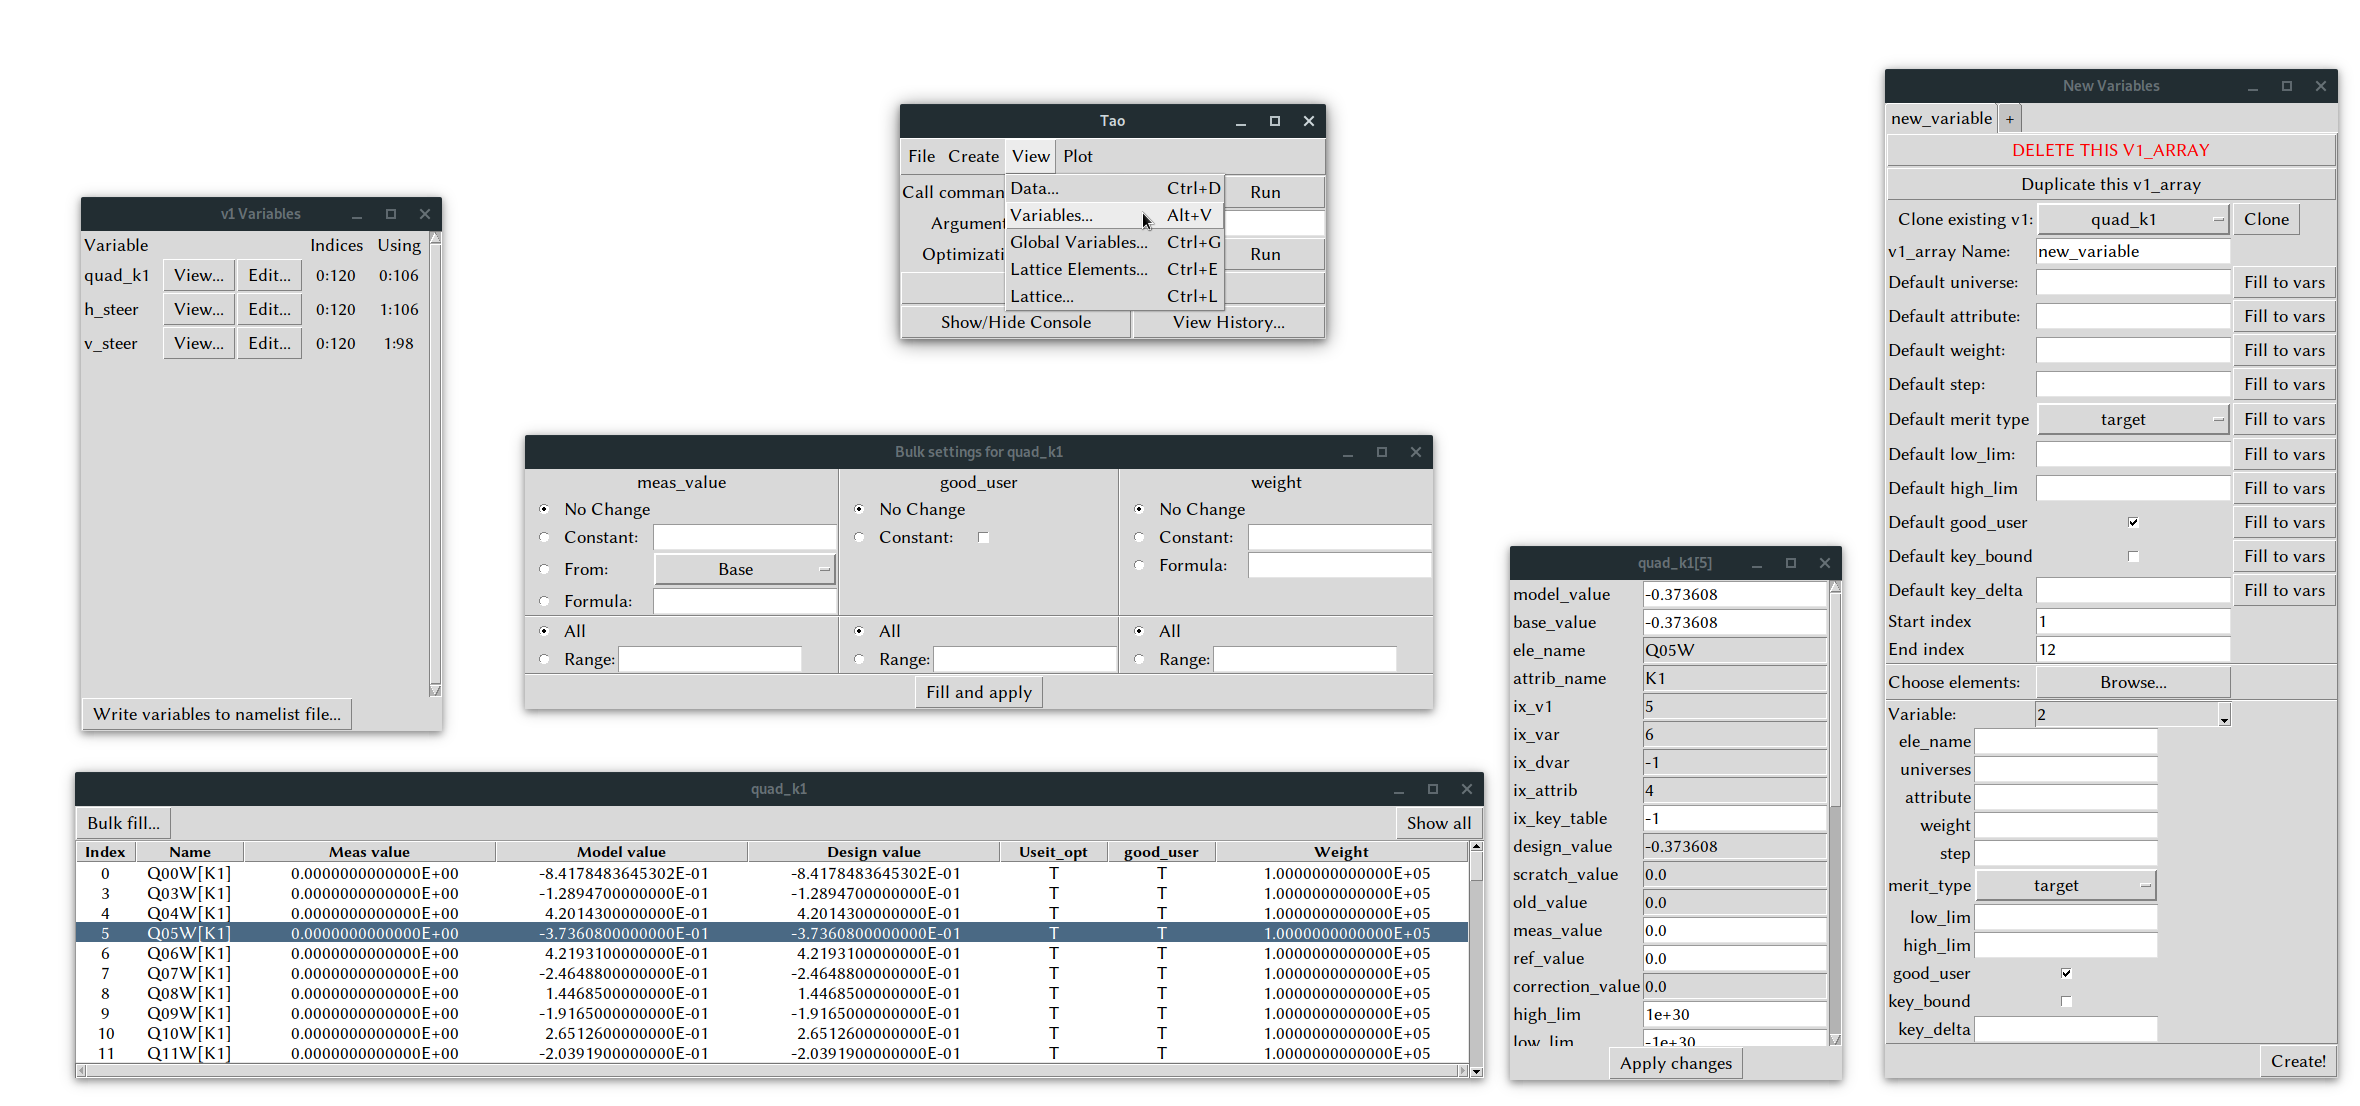
\includegraphics[width=12cm]{figures/variables.png}
\caption{The variable viewing and editing windows in the GUI.
Top middle: accessing the v1 variable window from the root window (console hidden).
Top left: the v1 variable window, showing the currently defined v1 variable arrays.
Bottom left: the variable window for quad_k1, displaying each of its variables and their key attributes.
Middle: the bulk fill window for quad_k1.
Bottom middle: the individual variable window for quad_k1[5], showing all of its settings and allowing the user to edit some of them.
Right: The variable array creation window.}
\label{fig:gui.variables}
\end{figure}
An important exception is that, since there are only v1 variables arrays and no v2 arrays of v1 arrays, the variable creation window only has one pane, and separate v1 arrays created in different tabs of the window are completely independent.
Also, the user can clone an existing v1 array with the drop down menu below the "Duplicate" button.

%-----------------------------------------------------------------
\section{Plotting}
\label{s:gui.plot}

One of the GUI's strong suits is the ability to view an manipulate plots using matplotlib.
Existing plots can be viewed and edited, and new templates can be defined on the fly.

Note: the GUI does support classic PG/PLplots, but it is recommended to use matplotlib as the plotting engine due to the extra fatures it offers.

\subsection{Viewing Plots}
\label{s:gui.plot.view}
Figure \ref{fig:gui.plot.view} shows how to plot existing templates in the GUI.
\begin{figure}
\centering
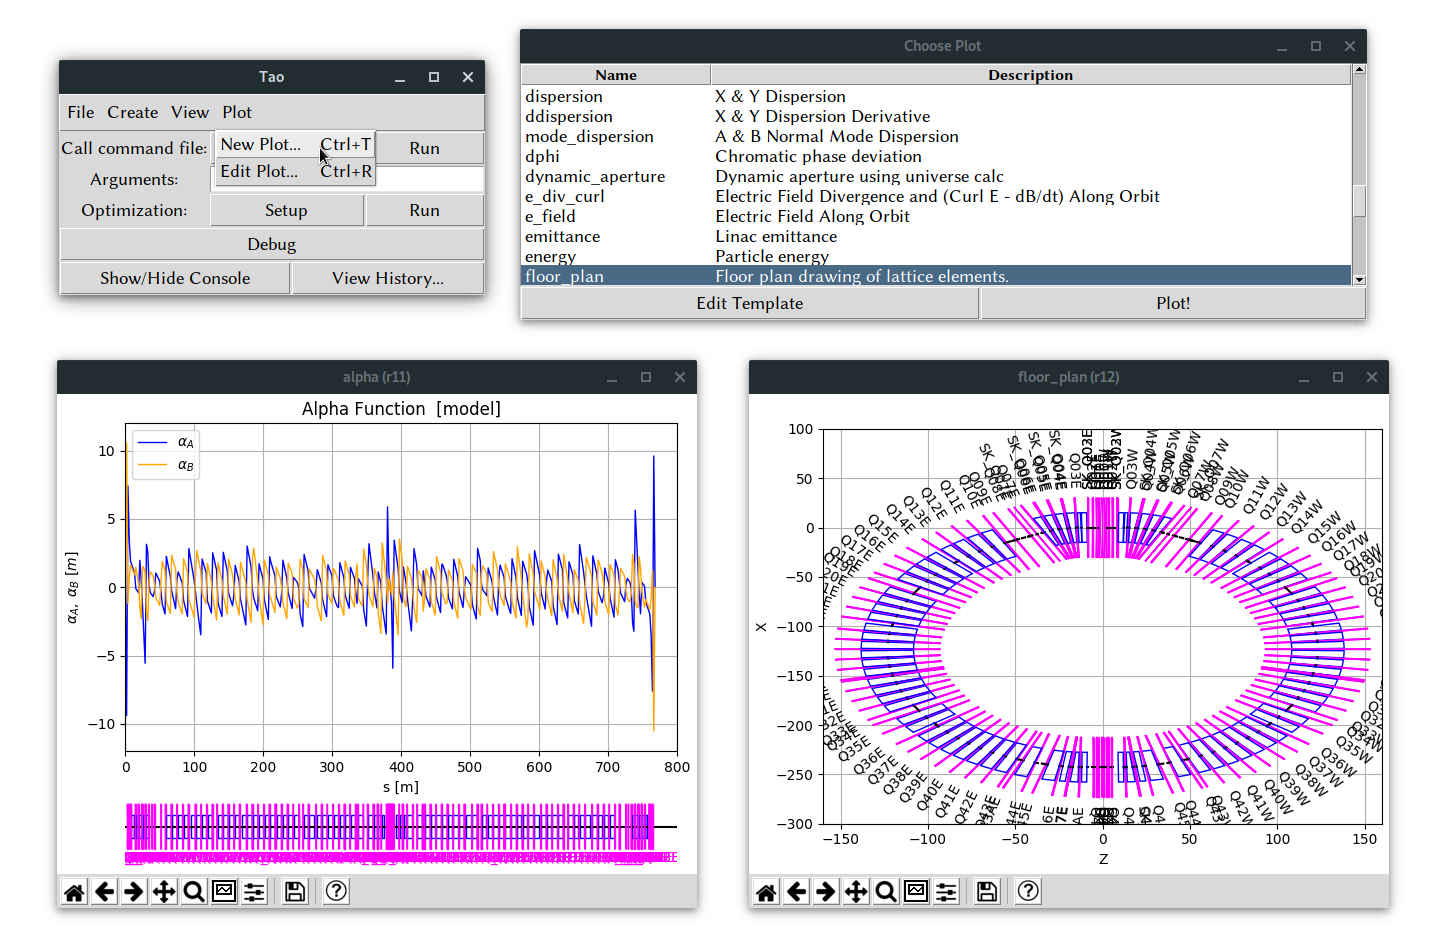
\includegraphics[width=12cm]{figures/view_plot.png}
\caption{Viewing plots with the GUI.
Top left: accessing the plot template list from the root window.
Top right: the plot template window.
Bottom left: a plot of the alpha function with the lat_layout shown below.
Bottom right: the floor_plan plot.}
\label{fig:gui.plot.view}
\end{figure}
The plot template window lists all of the currently defined plot templates as well as their descriptions.
A template can be plotted either by double clicking on it, or by selecting it and then clicking the "Plot" button.
This will open a window displaying the selected plot (see Section \ref{s:gui.plot.interaction} for more information).
The user can also edit an existing template by selecting it in the tempalte window and clicking "Edit Template".


\subsection{Interacting with Plots}
\label{s:gui.plot.interaction}
Interacting with plots in the GUI is primarily done using the toolbar along the bottom of the plotting window.

Starting from the left, the home button returns the graph to the starting view. The back button returns to the previous view of the graph, working as an undo button. The forward button undoes the effects of the back button. All of these buttons also have keyboard shortcuts, 'h' or 'r' for home, 'c' or 'left arrow' for back, and 'v' or 'right arrow' for forward.

The pan/zoom button allows panning of the graph by holding a left click on the graph and dragging the mouse around. his mode also allows zooming of the graph by holding a right click on the graph and dragging the mouse around. These actions can be restricted to the horizontal axis by holding 'x' while dragging, or the vertical axis by holding 'y'. Holding 'control' while dragging the mouse will preserve aspect ratio. Clicking on the toolbar button again will get out of this mode.

The zoom to rectangle button allows a rectangle to be selected by holding a left click on the graph and dragging the mouse, which will then fill the graph window. Holding 'x' or 'y' while selecting a rectangle will only effect the horizontal or vertical axis respectively.

The save button allows the graph window to be saved as an image file. Using 'ctrl+s' has the same effect.

If any floor plan or lat layout is present, double clicking on an element will open a window to view or edit element parameters.

Floor plans contain a slider to scale the size of elements away from the element centerline. Clicking on the slider will adjust the width of the displayed elements.

%-----------------------------------------------------------------
\subsection{Plotting Initialization}
\label{s:gui.plot.init}

When operating the GUI in matplotlib mode, you can specify a list of template plots to plot in matplotlib as soon as tao starts.  These templates should be listed in a file called plot.gui.init, which should be in the same directory from which you launch the gui.

plot.gui.init should have one template listed per line and absolutely nothing else on the line.  The templates listed in plot.gui.init are checked against the list of templates that tao can plot, and if a template is not recognized it is simply ignored.


%-----------------------------------------------------------------
\section{Lattice Elements}
\label{s:gui.lat}
\subsection{Lattice Templates}
\label{s:gui.lat.templates}

You can save your settings from the lattice table window in a template file, which can then be loaded and added to from within the gui.
The file can be named anything, and the formatting is as follows:
Lines starting with \# are considered comments and ignored.
Lines starting with "name:" are interpreted as a name for the settings listed in the line directly below
All other lines are interpreted as switches, as would be used with the show lattice command in Tao (see the tao manual for more info).
All switches for a given template should be on one line.

Example:
\begin{example}
#MY TEMPLATE FILE
name:template 1
-orbit -spin -tracking_elements
name:template 2
-lords q*
name: another template
-floor_coords -s 10:20
-radiation_integrals -all
\end{example}

This template file defines four templates: "template 1", "template 2", "another template", and an unnamed template (which has the switches -radiation_integrals -all).  Named templates are displayed by name in the gui, while unnamed templates are simply displayed by what switches they specify.

%-----------------------------------------------------------------
\section{Writing Namelists}
\label{s:gui.namelist}
